\documentclass{article}
\usepackage{graphicx} % Required for inserting images
\usepackage{amsmath}
\usepackage{mathtools}
\usepackage[a4paper, total={6in, 8in}]{geometry}
\usepackage{hyperref}
\usepackage{xcolor}
\usepackage{float}

\DeclareMathOperator*{\argmax}{arg\,max}
\DeclareMathOperator*{\argmin}{arg\,min}
\DeclarePairedDelimiterX{\verticalbar}[2]{[}{]}{%
  #1\;\delimsize\|\;#2%
}

\newcommand{\KL}[2]{\mathrm{KL} \verticalbar*{#1}{#2} }  % KL-divergence
\newcommand{\Q}{\textcolor{red}{\textbf{Question: }}}
\newcommand{\todo}{\textcolor{blue}{\textbf{TODO }}}

\title{Representational coarse-graining from limits on observation}

%\author{Johannes Valentinus Andreae}

\begin{document}
\maketitle

This project came about as part of a broader research effort aiming to develop a computational tool that can be used to model representational dynamics; that is, the meta-cognitive choices learning agents continually make about what information they ought to retain from their sensory streams to make decisions\footnote{ People mean all sorts of things when they say representation. This is mostly fine, but I'd like to address one particular criticism, which is that of 80s representationalism, brought forward by e.g. Hubert Dreyfus, Rodney Brooks, as well as David Chapman and Phil Agre\cite{agre1987pengi}. Chapman in one of his essays says (paraphrased from memory, seems to have vanished from cyberspace) that positing mental representations that have a correspondence to real-world objects is nonsense, and the word itself has no useful meaning besides the very boring one of a thermostat ``representing" the world via the angle of its bimetal rod. While I agree that positing correspondence is nonsensical, but what I mean by representation is exactly the thermostat thing, and I argue that if you allow the thermostat to be reasonably complex, then the representation becomes the set of intermediary variables that connect sensation to decision, and it is the opposite of boring to characterise the flow of information between these domains. This is also related to the stance of e.g. Maturana and Varela which I discuss in Section \ref{seq:autopoiesis}.}. I believe representational dynamics to be the backbone of any intelligent behaviour, and to encompass e.g. concept formation, belief changes and all what is interesting about human cognition. My approach is concerned with three major aspects of this dynamic: first, setting frames, in the sense of choosing the model in which to make inferences\footnote{The original frame problem is defined in terms of predicate logic, but here I mean it more generally, to choose any and all properties of a mathematical model to start solving an inference problem with (regardless of those being about some immediate state of the world or choice or some structural property of the environment, e.g. causal structure), in a big world\cite{javed2024big}.}, second, the actual temporal dynamics of the framing choices over the course of a learning process, and third, task switching in the sense of the agent realising that it should solve a related but different task to what it's currently solving (e.g. one at a much coarser granularity in terms of choices), based on a meta-cognitive evaluation of its situation and performance\footnote{This is a major point in Hofstadter's G\"odel, Escher, Bach\cite{hofstadter1999godel} - he proposes that intelligence is basically being able to make such realisations and switches, and I tend to agree.}.

The direct antecendent of this project within the above program is the one about representational planning\footnote{Fragments survive on cuneiform tablets unearthed at the construction of the new MPI-BC cafeteria building\cite{banyai2022forking, shen2023meta}} (RP - I discuss the exact relationship between the two approaches in detail in Section \ref{sec:rp_vs_mi}). RP proved to be very useful to define representational dynamics very generally and normatively within the framework of reinforcement learning (RL), and also to establish a basic relationship between representational complexity and some task properties. At the same time, it proved very difficult to work with in terms of computational requirements due to a combinatorial explosion in the number of possible representational updates throughout learning, and also the ability to produce compact principles for these updates. Thus, it was reasonable to look for an alternative lens that can be used in simplified situations to arrive at such a principle, but can still be interestingly connected to the general problem. It turns out that if we are willing to use information theory instead of RL, then rate-distortion theory gives us normative representational coarse-graining for free. Let's see how we can arrive to a setting in which this can be applied to our questions. 

\section{Frame from finitude}

A simpler scenario in which the frame problem applies just as well is passive statistical learning, usually modelled as Bayesian inference (BI). However, in order to constrain any property of the model itself beyond the posterior BI would result in, one will need to use an additional piece of information about the learning scenario. One such possibility arises from the fact that a learner typically has a sense of how quickly it has to acquire the learning target, either due to external pressure, e.g. every new observation carrying additional risk, or an internal one, e.g. having to acquire food before starvation sets in. This urgency is importantly different from urgency within a single trial, where the amount of computation the agent can do on the sensory input before making a decision is limited (e.g. how precisely we can position the ping-pong racket before the ball gets too close), as in our case the urgency is applied to the entire learning process (e.g. we know we have about 20 games to get good enough at ping-pong so that the other kids don’t get frustrated playing with us)\footnote{For Bayesian learners, this piece of information from the task definition is extraneous to usual formalisations of the learning problem, while in RL it is always part of the task definition in the form of a horizon or a discount factor.}. This extra constraint won't solve us the entire frame problem, but it will solve a small slice of it, namely when we have a set of candidate variables, which possible values should we consider for those a priori. 

\subsection{The finite-data mutual information objective}
The basic mathematical result on which the project is built is summarised in \cite{mattingly2018}, and states that one can choose the prior for an inference problem such that it maximises the expected number of bits we will learn from a set number of observations (the main result is actually an older one from rate-distortion theory\cite{rose2002mapping}). Formally stated, in an inference problem where the latent parameter $\theta$ has to be estimated using a known number $n$ of observations $x$, related to the latent by the known likelihood function $p_{x \mid \theta}$, the optimal prior is given by: 

\begin{equation}
    p^*(\theta \mid n, p_{x \mid \theta}) = \argmax_{p(\theta)} I(\theta, \lbrace x_1 \ldots x_n \rbrace)
\end{equation}

where $I$ is mutual information (MI)\footnote{This is the definition of the reference prior of Bernardo, adapted for a finite number of future observations. As $n \rightarrow \infty$, it will converge to the actual reference prior, which often coincides with the Jeffreys prior.}. This is a convex objective, that can be optimised by the Blahut-Arimoto algorithm (BA - specific steps given in Section \ref{sec:ba_mi})\footnote{Further caluclations and simulations can be found in \href{https://github.com/mihalybanyai/infomax/blob/main/sequential_infomax.ipynb}{this notebook}. }. 

This is obviously very relevant, as such a prior is part of the definition of the model in which inference is conducted, thus part of the representation of the agent. Furthermore, the $p^*$ coming out of the BA is very often, under mild assumptions discrete, without having this discreteness injected as an assumption or the consequence of e.g. choosing actions\footnote{Building intuition about why exactly this discreteness arises is not straightforward though. The finite number of bits certainly have a role, and so do the existence of special points, e.g. ends of the interval over which $\theta$ is supported (discreteness doesn't arise e.g. for a Gaussian-distributed $\theta$ over an infinite support, which is probably one reason this result is not more widely known). Game theoretic reformulations of the inference problem are said to help. I'm still on the fence whether I need better intuition about the underlying reasons here.}. And as the discrete atoms in the support of the prior correspond to intervals that are coarse-grained into the atoms, we get a very neat representational space in which complexity is straightforwardly defined and normatively determined by the resource constraint\footnote{This turned out to be one of those situations when a result is so obviously relevant that it seems unbelievable that it's not more widely applied. And while it is applied in some disciplines, e.g. economics\cite{jung2019discrete}, physics\cite{shamai1990capacity}, immunology\cite{mayer2015well} and even neural population coding\cite{bethge2003optimal, nikitin2009neural, shao2023efficient}, it is far from universally acknowledged, especially in computational cognitive science, especially given its potential significance.}. 

Of course, the result is also limited in multiple ways - having to know $n$ \emph{exactly} doesn't really correspond to what situated agents actually know about the urgency of their learning problem. The objective is also one-shot, instead of addressing a sequential decision making situation. I try to address both of these problems by extending the basic result to sequential situations in Section \ref{sec:dynamics}, as well as the case when the likelihood function isn't fully known in advance. 

Then I will address how the MI as the objective can follow from the RP setting in special cases, instead of having to assume the information theoretic objective as fundamental. This is also important in order to clarify what information-theoretic optimality means for task performance under various environmental conditions. With such an optimisation, several other existing frameworks spring to mind immediately, such as resource rationality or efficient coding, to which I address the relationship in Section \ref{sec:others}.


\section{Dynamics} \label{sec:dynamics}
\subsection{How to combine past and future?}

If the learning is not one shot, but is situated in a sequential setting, the most elementary operation we need is to make a representational choice when we already have learned information from a set of $m$ old observations, $X_{old}$, that we discarded when inferring $\theta_{old}$. Then we have this source of information together with the new set of $n$ observations, $X$, as depicted in Fig. \ref{fig:info_venn}.

\begin{figure}[H]
    \centering
    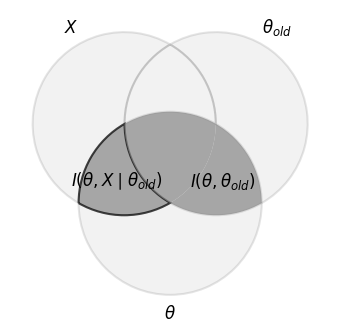
\includegraphics[width=0.5\textwidth]{info_venn.png}
    \caption{The Venn diagram of the variables determines the decomposition of the information we want to incorporate into $\theta$.}
    \label{fig:info_venn}
\end{figure}

So we arrive to the optimisation problem in Eq. \ref{eq:past_future_opt}. 

\begin{equation}\label{eq:past_future_opt}
    p^*(\theta \mid n, p_{x \mid \theta}, X_{old}) = \argmax_{p(\theta)} I(\theta, \theta_{old}) + I(\theta, X \mid \theta_{old})
\end{equation}

A technical trick to compute the MI, decribed in Eq. \ref{eq:samping}, involves sampling synthetic observations according to the old estimate $\theta_{old}$ \footnote{This step was indeed introduced out of technical considerations, but actually it creates a possibility to seamlessly integrate episodic memories into the calculation.}. 

\begin{equation}\label{eq:samping}
    \tilde{x} \sim p(\tilde{x}) = \sum_{\theta_{old} \in \Theta} p(\tilde{x} \mid \theta_{old}) p(\theta_{old} \mid X_{old})
\end{equation}

Then the objective function for maximising the combination of past and future information ends up being Eq. \ref{eq:dynamic_objective}, for which the derivation is given in Section \ref{sec:dyn_obj}. 

\begin{equation}\label{eq:dynamic_objective}
    \mathcal{L}_{dyn} \approx \argmax_{p(\theta)} \sum_{\theta \in \Theta} p(\theta) \frac{1}{m}\sum_{s=1}^m p(\tilde{x}_s \mid \theta)  \left[ \log \frac{p(\tilde{x}_s \mid \theta)}{p_{new}(\tilde{x}_s)} + \sum_{X \in \mathcal{X}^n} p(X \mid \theta) \log \frac{p(X \mid \theta)}{p(X)} \right]
\end{equation}

Trying out the BA for this objective on a toy setting with a biased coin is depicted in Fig. \ref{fig:dynamic_opt}. We can see that the basic behaviour of the algorithm is that the support of the optimal prior is determined by what we expect in the future, and the probability masses assigned to the atoms in the support is determined by the pre-existing posterior. This result can be regarded as intuitive, as it's the future question that should determine the formalisation of the learning problem more, but this requires further thought whether the result is admissible as is.

\begin{figure}[h]
    \centering
    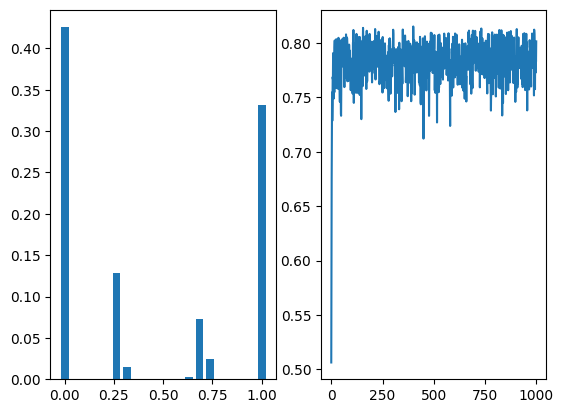
\includegraphics[width=0.7\textwidth]{dynamic_opt.png}
    \caption{Left: $p*$. Right: the value of Eq. \ref{eq:dynamic_objective} over time}
    \label{fig:dynamic_opt}
\end{figure}

\Q what do I have to do for the interaction between past and future terms to play out differently? What about the version that handles uncertainty in $n$?

\subsection{The daisy chain}

Once we have an optimisation step that ties past and future together, this can sit in the middle of a sequence of updates, we can try to construct a process model of learning that involves meta-cognitive representational updates. This is very much a work in progress, but the first iteration to do so is illustrated in Fig. \ref{fig:daisy_chain}. The important observation here is when optimising the MI objective, we automatically get an estimate of how much we expect to learn from the incoming observations, which is the MI itself (or rather its future-only component). This is basically a measure of how correct our assumptions were, and our main assumption was the for of the likelihood function. Thus, if the estimated amount of learning turns out to be way off, then we can use this as a signal to rectify the likelihood function. This way we create a feedback loop that continually evolves both the representation and the likelihood of the agent in a combination of representational updates and efficient coding updates (this connection is elaborated upon in Section \ref{sec:ec}).

\begin{figure}[h]
    \centering
    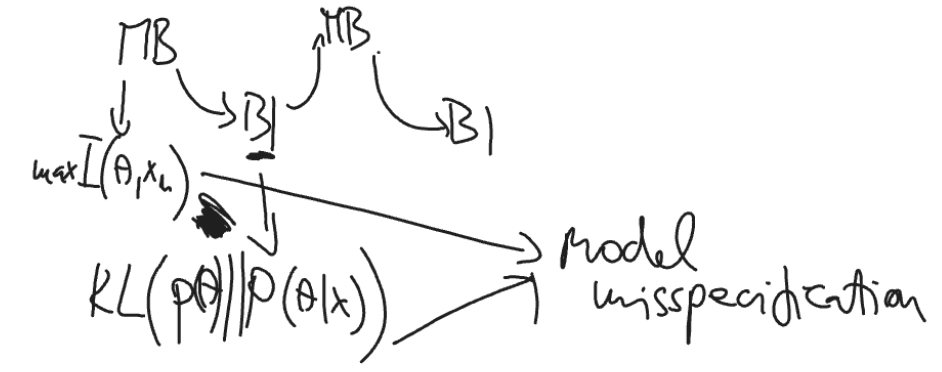
\includegraphics[width=0.7\textwidth]{misspec_signal.png}
    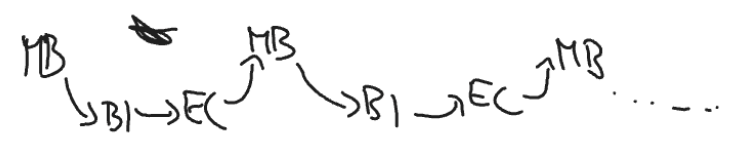
\includegraphics[width=0.7\textwidth]{daisy.png}
    \caption{MB here refers to the representational choice that is made by optimising Eq. \ref{eq:dynamic_objective} (it stands for ``model building"). \textbf{Top}: It is being alternated by the actual learning via BI, which produces the model misspecification signal as the discrepancy between the expected number of learned bits calculated in the MB step and the actual number of learned bits at the end of the BI step.
    \textbf{Bottom}: The BM and BI steps are also alternated with an EC step adjusting the likelihood based on the misspecification signal.}
    \label{fig:daisy_chain}
\end{figure}

\Q what is the name for this kind of model which is not normative, as there is no closed-form objective it maximises, but it's a feedback loop operating on some signal. All sorts of replicator dynamics should be in this category, as well as the objective-haters' (Stanley and Clune) open-ended dynamics, and of course Maturana's autopoiesis, and the modern algorithm-haters' version of it

\subsection{Computational complexity}

When looking for an alternative computational framework to one that was too computationally expensive, having to continually re-optimise MIs is not the slam dunk one would hope for. Consequently, looking for nicely behaving approximate and amortised solutions is in order.

\todo The particle filter option to compute MIs\cite{dauwels2005numerical}.


\section{How is this a special case of the general case?}\label{sec:rp_vs_mi}

\todo write this section

\subsection{Representational planning}

Described to some degree in \cite{banyai2022forking, shen2023meta}.

\subsection{Passive-informational MDPs}

\begin{itemize}
    \item BA is convex. Under what circumstances is value estimation through planning convex? I the inside loop of root sampling convex?
    \item when the task \emph{is} learning, then the value of information ought to correspond to all value - as in VAEs vs. the IB, where if the IB rhs variable is the same as the lhs one, you get back a VAE
    \item MI is akin to the finite horizon planning, and then the Jeffreys would be the asymptotic one? but with what choice for a discount factor (or maybe it isn’t exponential discounting)?
    \item the learning task remove the temporal contingencies, so it's contextual bandit
    \item there was a point about non-Markovian thresholds in the reward function infuencing representational choices in \cite{shen2023meta} (possibly only in the \href{https://github.com/mihalybanyai/infomax/blob/main/ccn2023_poster_replan2.pdf}{poster version}), and this is probably strongly related to both limited information and satisficing\cite{arumugam2021deciding}
    \item inference-as-planning \cite{buesing2020}
    
\end{itemize}

\subsection{Optimality and evaluation}

The amount of stochasticity in the environment seems paramount here\footnote{Simulations of coin toss environments in \href{https://github.com/mihalybanyai/infomax/blob/main/infomax_class.py}{this notebook}}, and it was also a parameter that greatly influenced representational coarse-graining, as explained in this completely unpublished \href{https://github.com/mihalybanyai/infomax/blob/main/LM_221130_beliefs_and_representations.pdf}{lab meeting talk}.

\Q How does exactly betting optimality depend on stochasticity and other task properties? 

\subsection{Discounting}

There was a strong influence of the discount factor and the planning horizon on representational choices in \cite{shen2023meta}, which seems analogous to the dependence on $n$ here.

\section{Relation to other approaches} \label{sec:others}

\todo write these out properly

\subsection{Hierarchical Bayesian inference}

\begin{itemize}
    \item The reason these all end up being heuristics is that they try to solve an issue that is outside of BI from within
    \item what does it mean to be outside? to use different information. RL is outside of BI because of the reward signal
    \item BI has this kinda flat view of the world, as one big statistician’s assignment, while there is a detailed agent-environment dynamic with boundaries and various constraints at play
    \item on top of the spatial structure of the boundaries, there is a lot of temporal structure too - the agents are doing tasks
\end{itemize}

\subsection{Resource rationality}

\begin{itemize}
    \item resource rationality does get at some of the additional structure
    \item  but it ends up focusing almost entirely on the agent’s internal architecture in terms of computational constraints
    \item which is fair, but I think it does end up being the less interesting side of the coin
    \item and while the other side, the task structure, is absolutely there in the mission statement, it ends up being neglected
    \item observational and computational costs are possible to transform into each other to some degree
    \item but there is a limit to that, you can't create information via computation
    \item and we often don't really know how to do the transformation; the cost of computing is notoriously difficult to either empirically assess or even theorise about
\end{itemize}

\subsection{Efficient coding} \label{sec:ec}

\begin{itemize}
    \item optimizes the same objective function in terms of the likelihood
    \item the instantaneus version\cite{mlynarski2022efficient} seems quite amenable to build into a process model 
\end{itemize}

\subsection{Autopoiesis}\label{seq:autopoiesis}

\begin{itemize}
    \item very agent-centric view, based on the notion of finitude, i.e. the agent is what is combatting its own decomposition
    \item different from autocathalitic and other self-reinforcing processes, because those don’t combat decomposition, as they burn through their fuel as fast as possible then die\cite{jaeger2024naturalizing}
    \item the algorithmic side is severely underdeveloped as one might have guessed
    \item helpfully, autopoets use “representation” to mean the opposite of what I mean by it
    \item related to open-endedness\cite{wang2020enhanced}
\end{itemize}

\subsection{Others}
\begin{itemize}
    \item Optimal stopping: when the urgency in information gathering manifests within a single trial
    \item Optimal experiment design: optimising the same objective in terms of $n$
    \item Affordances: they are the mirror image of representations. What an MI-maximising agent does is to basically construct an affordance for the environment to use on itself (cf. \cite{abel2025plasticity})
    \item Risk sensitivity: risk is not the same as urgency, but it's one way to have it
    \item Bias-variance dilemma: it's not really a dilemma, but in any case observational limitations put us into a special case of it
    \item Active learning: optimising the same objective in terms of the data
    \item \Q are there other fields I have to relate to?
\end{itemize}

\section{How to use these tools to model specific learning situations?}

\todo All the nitty-gritty of matching the maths to an experimental design.

\appendix

\section{Glossary}

\begin{itemize}
    \item BA - Blahut-Arimoto algorithm
    \item BI - Bayesian inference
    \item EC - efficient coding theory
    \item MI - mutual information
    \item RL - reinforcement learning 
    \item RP - representational planning
    \item RR - resource rationality
\end{itemize}

\section{Derivations and algorithms}

\subsection{Blahut-Arimoto updates for the MI objective} \label{sec:ba_mi}

As per \cite{mattingly2018}.

\begin{eqnarray}
    p_{\tau+1}(\theta) = \frac{1}{Z_\tau} e^{\KL{p(X \mid \theta)}{p(X)}} p_\tau(\theta) \\
    Z_\tau = \sum_{\theta \in \Theta} e^{\KL{p(X \mid \theta)}{p(X)}} p_\tau(\theta)
\end{eqnarray}

\subsection{Derivation of the dynamic objective function} \label{sec:dyn_obj}

In the case of trying to choose an optimal $p^*(\theta)$ repeatedly, we would want to maximise the MI between all past and future observations simultaneously. However, as individual past observations are not retained, all information about those is in the posterior distribution $p(\theta_{old} \mid X_{old})$, where $X_{old} \in \mathcal{X}^m$, estimated from $m$ observations, with the likelihood function remaining the same. The resulting MI maximisation is illustrated in the above Venn-diagram, and 

\begin{equation}
    p^*(\theta \mid n, p_{x \mid \theta}, X_{old}) = \argmax_{p(\theta)} \mathcal{L}_{dyn} = \argmax_{p(\theta)} I(\theta, \theta_{old}) + I(\theta, X \mid \theta_{old})
\end{equation}

\subsubsection{Projecting the posterior into observation space}

For this objective to be completely defined, we'd need $p(\theta, \theta_{old} \mid n, m)$ to be defined. We'd like to avoid giving such a definition for now, and sidestep the problem by introducing a variable for synthetic observations, and assume it to be connected to the latent via the same likelihood function we used so far:

\begin{equation}
    \tilde{x} \sim p(\tilde{x}) = \sum_{\theta_{old} \in \Theta} p(\tilde{x} \mid \theta_{old}) p(\theta_{old} \mid X_{old})
\end{equation}

Then we make the following equivocation in the objective function, making it completely defined, albeit not in a way that makes the balancing effect of $n$ and $m$ explicit, to which we will come back later:

\begin{equation}
    \mathcal{L}_{dyn} = \argmax_{p(\theta)} I(\theta, \tilde{x}) + I(\theta, X \mid \tilde{x})
\end{equation}

\subsubsection{The future term}

The conditional term is slightly easier to handle, so let's look at that first:

\begin{equation}
    I(\theta, X \mid \tilde{x}) = \sum_{\tilde{x} \in \mathcal{X}} p(\tilde{x}) \sum_{\theta \in \Theta} p(\theta \mid \tilde{x}) \sum_{X \in \mathcal{X}^n} p(X \mid \theta, \tilde{x}) \log \frac{p(X \mid \theta, \tilde{x})}{p(X \mid \tilde{x})}
\end{equation}

Here we observe that $\theta$ is a Markov blanket between $X$ and $\tilde{x}$, thus $p(X \mid \theta, \tilde{x}) = p(X \mid \theta)$ and $p(X \mid \tilde{x}) = \sum_{\theta \in \Theta} p(X \mid \theta, \tilde{x}) p(\theta) = p(X)$.

Then we expand the conditional: 

\begin{equation}
    p(\theta \mid \tilde{x}) = \frac{p(\tilde{x} \mid \theta) p(\theta)}{\sum_{\theta \in \Theta} p(\tilde{x} \mid \theta) p(\theta)}
\end{equation}

Then introduce the shorthand $p_{new}(\tilde{x}) = \sum_{\theta \in \Theta} p(\tilde{x} \mid \theta) p(\theta)$, so the conditional MI becomes:

\begin{equation}
    I(\theta, X \mid \tilde{x}) = \sum_{\tilde{x} \in \mathcal{X}} p(\tilde{x}) \sum_{\theta \in \Theta} \frac{p(\tilde{x} \mid \theta)}{p_{new}(\tilde{x})} p(\theta) \sum_{X \in \mathcal{X}^n} p(X \mid \theta) \log \frac{p(X \mid \theta)}{p(X)}
\end{equation}

\subsubsection{The sampling trick}

At this point we'd like to reintroduce the consideration that $m$ (or at least the ratio between it and $n$) should play a role in how much information do we actually copy from the posterior into the new prior. We do this by taking $m$ samples from $p(\tilde{x})$, and calculate the expectation using those:

\begin{equation}
    \tilde{x}_1 \ldots \tilde{x}_m \sim p(\tilde{x})
\end{equation}

\begin{eqnarray}
    I(\theta, X \mid \tilde{x}) \approx \frac{1}{m}\sum_{s=1}^m \sum_{\theta \in \Theta} \frac{p(\tilde{x}_s \mid \theta)}{p_{new}(\tilde{x}_s)} p(\theta) \sum_{X \in \mathcal{X}^n} p(X \mid \theta) \log \frac{p(X \mid \theta)}{p(X)} = \\
    = \sum_{\theta \in \Theta} p(\theta) \left[ \frac{1}{m}\sum_{s=1}^m \frac{p(\tilde{x}_s \mid \theta)}{p_{new}(\tilde{x}_s)} \right]  \sum_{X \in \mathcal{X}^n} p(X \mid \theta) \log \frac{p(X \mid \theta)}{p(X)}
\end{eqnarray}

This approximation can be done fully stochastically as stated here, or if we retained any real observations in episodic memory, we can use those as well.

\subsubsection{The past term}

In order to be able to use the same set of samples for approximation, we expand the non-conditional term in the less intuitive way:

\begin{equation}
    I(\theta, \tilde{x}) =  \sum_{\tilde{x} \in \mathcal{X}} p(\tilde{x}) \sum_{\theta \in \Theta} p(\theta \mid \tilde{x}) \log \frac{p(\theta \mid \tilde{x})}{p(\theta)} = 
    \sum_{\tilde{x} \in \mathcal{X}} p(\tilde{x}) \sum_{\theta \in \Theta} \frac{p(\tilde{x} \mid \theta) p(\theta)}{p_{new}(\tilde{x})} \log \frac{p(\tilde{x} \mid \theta)}{p_{new}(\tilde{x})}
\end{equation}


Then using the samples this becomes:

\begin{equation}
    I(\theta, \tilde{x}) \approx  \sum_{\theta \in \Theta} p(\theta) \frac{1}{m}\sum_{s=1}^m \frac{p(\tilde{x}_s \mid \theta)}{p_{new}(\tilde{x}_s)}  \log \frac{p(\tilde{x}_s \mid \theta)}{p_{new}(\tilde{x}_s)}
\end{equation}

\subsubsection{The full objective}

From all the above it seems the full objective would be:

\begin{equation}
    \mathcal{L}_{dyn} \approx \argmax_{p(\theta)} \sum_{\theta \in \Theta} p(\theta) \frac{1}{m}\sum_{s=1}^m  \frac{p(\tilde{x}_s \mid \theta)}{p_{new}(\tilde{x}_s)}  \left[ \log \frac{p(\tilde{x}_s \mid \theta)}{p_{new}(\tilde{x}_s)} + \sum_{X \in \mathcal{X}^n} p(X \mid \theta) \log \frac{p(X \mid \theta)}{p(X)} \right]
\end{equation}

But it is also very obvious from the gestalt of KL divergences in general that this formula wants to be 

\begin{equation}
    \mathcal{L}_{dyn} \approx \argmax_{p(\theta)} \sum_{\theta \in \Theta} p(\theta) \frac{1}{m}\sum_{s=1}^m  p(\tilde{x}_s \mid \theta)  \left[ \log \frac{p(\tilde{x}_s \mid \theta)}{p_{new}(\tilde{x}_s)} + \sum_{X \in \mathcal{X}^n} p(X \mid \theta) \log \frac{p(X \mid \theta)}{p(X)} \right]
\end{equation}

And this is indeed empirically validated by the simulations being a lot more reasonable this way. 
\Q What derivation step am I missing here?

\subsubsection{Blahut-Arimoto updates}

since $I(\theta,  \left[X, \tilde{x} \right]) = \sum_{\theta \in \Theta} p(\theta) \KL{p(X, \tilde{x} \mid \theta)}{p(X, \tilde{x})}$, from the above it is obvious that 

\begin{equation}
   \KL{p(X, \tilde{x} \mid \theta)}{p(X, \tilde{x})} = \frac{1}{m}\sum_{s=1}^m  p(\tilde{x}_s \mid \theta) \left[ \log \frac{p(\tilde{x}_s \mid \theta)}{p_{new}(\tilde{x}_s)} + \sum_{X \in \mathcal{X}^n} p(X \mid \theta) \log \frac{p(X \mid \theta)}{p(X)} \right] 
\end{equation}

this can be used to implement a Blahut-Arimoto iteration to find $p^*(\theta \mid n, p_{x \mid \theta}, X_{old})$ similarly to the static case:

\begin{eqnarray}
    p_{\tau+1}(\theta) = \frac{1}{Z_\tau} e^{\KL{p(X, \tilde{x} \mid \theta)}{p(X, \tilde{x})}} p_\tau(\theta) \\
    Z_\tau = \sum_{\theta \in \Theta} e^{\KL{p(X, \tilde{x} \mid \theta)}{p(X, \tilde{x})}} p_\tau(\theta)
\end{eqnarray}

\begin{eqnarray}
    p_{\tau+1}(\theta) = \frac{1}{Z_\tau} e^{\KL{p(X \mid \theta)}{p(X)}} p_\tau(\theta) \\
    Z_\tau = \sum_{\theta \in \Theta} e^{\KL{p(X \mid \theta)}{p(X)}} p_\tau(\theta)
\end{eqnarray}

\bibliographystyle{plain}
\bibliography{infomax_refs}

\end{document}
